\documentclass[12pt, a4paper, twoside]{scrartcl}
 %---- Allgemeine Layout Einstellungen ------------------------------------------

% Für Kopf und Fußzeilen, siehe auch KOMA-Skript Doku
\usepackage[komastyle]{scrpage2}
\pagestyle{scrheadings}
\setheadsepline{0.5pt}[\color{black}]


%Einstellungen für Figuren- und Tabellenbeschriftungen
\setkomafont{captionlabel}{\sffamily\bfseries}
\setcapindent{0em}


%---- Weitere Pakete -----------------------------------------------------------
% Die Pakete sind alle in der TeX Live Distribution enthalten. Wichtige Adressen
% www.ctan.org, www.dante.de

% Sprachunterstützung
\usepackage[ngerman]{babel}

% Benutzung von Umlauten direkt im Text
% entweder "latin1" oder "utf8"
\usepackage[utf8]{inputenc}

% Pakete mit Mathesymbolen und zur Beseitigung von Schwächen der Mathe-Umgebung
\usepackage{latexsym,exscale,stmaryrd,amssymb,amsmath}

% Weitere Symbole
\usepackage[nointegrals]{wasysym}
\usepackage{eurosym}

% Anderes Literaturverzeichnisformat
%\usepackage[square,sort&compress]{natbib}

% Für Farbe
\usepackage{color}

% Zur Graphikausgabe
%Beipiel: \includegraphics[width=\textwidth]{grafik.png}
\usepackage{graphicx}

% Text umfließt Graphiken und Tabellen
% Beispiel:
% \begin{wrapfigure}[Zeilenanzahl]{"l" oder "r"}{breite}
%   \centering
%   \includegraphics[width=...]{grafik}
%   \caption{Beschriftung} 
%   \label{fig:grafik}
% \end{wrapfigure}
\usepackage{wrapfig}

% Mehrere Abbildungen nebeneinander
% Beispiel:
% \begin{figure}[htb]
%   \centering
%   \subfigure[Beschriftung 1\label{fig:label1}]
%   {\includegraphics[width=0.49\textwidth]{grafik1}}
%   \hfill
%   \subfigure[Beschriftung 2\label{fig:label2}]
%   {\includegraphics[width=0.49\textwidth]{grafik2}}
%   \caption{Beschriftung allgemein}
%   \label{fig:label-gesamt}
% \end{figure}
\usepackage{subfigure}

% Caption neben Abbildung
% Beispiel:
% \sidecaptionvpos{figure}{"c" oder "t" oder "b"}
% \begin{SCfigure}[rel. Breite (normalerweise = 1)][hbt]
%   \centering
%   \includegraphics[width=0.5\textwidth]{grafik.png}
%   \caption{Beschreibung}
%   \label{fig:}
% \end{SCfigure}
\usepackage{sidecap}
\usepackage{float}

% Befehl für "Entspricht"-Zeichen
\newcommand{\corresponds}{\ensuremath{\mathrel{\widehat{=}}}}
\newcommand{\folgt}{\ensuremath{\mathrel{\Rightarrow}}}
\newcommand{\equals}{\ensuremath{\mathrel{\Leftrightarrow}}}
\newcommand{\degree}{\ensuremath{\mathrel{^{\circ}}}}

\newcommand{\nn}{\nonumber}
\newcommand{\tn}[1]{\textnormal{#1}}
\newcommand{\D}{\ensuremath{\mathrel{\rm d}}}

\newcommand{\const}{\tn{const}}

\newcommand{\meter}{\ensuremath{\mathrel{\tn m}}}
\newcommand{\kilogramm}{\ensuremath{\mathrel{\tn{kg}}}}
\newcommand{\second}{\ensuremath{\mathrel{\tn s}}}
\newcommand{\sekunde}{\second}

\newcommand{\volt}{\ensuremath{\mathrel{\tn V}}}
\newcommand{\pascal}{\ensuremath{\mathrel{\tn{Pa}}}}
\newcommand{\coulomb}{\ensuremath{\mathrel{\tn C}}}
\newcommand{\newton}{\ensuremath{\mathrel{\tn N}}}
\newcommand{\liter}{\ensuremath{\mathrel{\tn l}}}
\newcommand{\celsius}{\ensuremath{\mathrel{\tn C}}}
\newcommand{\fahrenheit}{\ensuremath{\mathrel{\tn F}}}
\newcommand{\joule}{\ensuremath{\mathrel{\tn J}}}
\newcommand{\kelvin}{\ensuremath{\mathrel{\tn K}}}
\newcommand{\mol}{\ensuremath{\mathrel{\tn{mol}}}}
\newcommand{\gramm}{\ensuremath{\mathrel{\tn{g}}}}

\newcommand{\kilo}{\ensuremath{\mathrel{\tn k}}}
\newcommand{\hecto}{\ensuremath{\mathrel{\tn h}}}

\newcommand{\centi}{\ensuremath{\mathrel{ \tn c}}}
\newcommand{\milli}{\ensuremath{\mathrel{ \tn m}}}
\newcommand{\micro}{\ensuremath{\mathrel{ \tn\mu }}}



%\newcommand{}{\ensuremath{\mathrel{  }}}
%\newcommand{}{\ensuremath{\mathrel{  }}}
%\newcommand{}{\ensuremath{\mathrel{  }}}


\newcommand{\person}[1]{\textsc{#1}}

 \begin{document}
 %Titelseite u. Inhaltsverzeichnis
\begin{titlepage}
\centering
\textsc{\Large Anfängerpraktikum der Fakultät für
  Physik,\\[1.5ex] Universität Göttingen}

\vspace*{4.2cm}

\rule{\textwidth}{1pt}\\[0.5cm]
{\huge \bfseries
  Spezifische Wärme der Luft und Gasthermometer}\\[0.5cm]
\rule{\textwidth}{1pt}

\vspace*{3.5cm}

\begin{Large}
\begin{tabular}{ll}
Praktikanten: &  Silke Andrea Teepe\\
& Marcel Kramer\\
E-Mail: & \\
Betreuer: & Alexander Schmelev\\
\end{tabular}
\end{Large}

\vspace*{0.8cm}

\begin{Large}
\fbox{
  \begin{minipage}[t][2.5cm][t]{6cm} 
    Testat:
  \end{minipage}
}
\end{Large}

\end{titlepage}
\cleardoublepage
\tableofcontents
\cleardoublepage
\setcounter{page}{1}

\section{Einleitung}
\label{sec:einleitung}

\section{Theorie}
\label{sec:theorie}

\subsection{Oberflächenspannung}
Der Effekt der Kapillarität wird von Wechselwirkungen auf molekularer Ebene verursacht. Diese können in Zwei Arten unterteilt werden. Zu einem in die Kohäsionskräften, die innerhalb der Flüssigkeit wirken und zum anderen in die Adhäsionskräften, Kräften die zwischen der Flüssigkeit und einem Festkörper (Glas) oder einem Gas (Luft) auftreten.\newline
\newline
Die wichtigsten Kohäsionskräfte sind die Van-der-Waals-Kräfte und die Dipol-Dipol-Kräfte. Die Van-der-Waals-Kräfte sind schwache Kräfte, die zwischen Molekülen und Atomen wirken. Sie entstehen durch zufällige Ladungsverschiebung innerhalb eines Moleküls durch seine freien Elektronen. Diese Ladungsverschiebungen verursachen, dass ein Molekül kurzzeitig zu einem Dipol wird und so mit anderen Molekülen wechselwirken kann. 
Dipol-Dipol-Kräfte hingegen werden zwischen Molekülen erzeugt, die ein dauerhaftes Dipolmoment besitzen.\newline
\newline
Hält man einen Festkörper in eine Flüssigkeit so entstehen zwischen den Molekülen der Flüssigkeit und den Molekülen des Festkörpers Adhäsionskräfte. Sind diese Adhäsionskräfte größer als die Kohäsionskräfte innerhalb der Flüssigkeit so kann man beobachten wie sich die Flüssigkeit am Rand des Festkörpers hochzieht. Dieser Effekt heißt Kapillarität und ist besonders gut zu beobachten, indem man ein Glaskapillare in Wasser hält. Man sieht wie sich das Wasser im Inneren der Kapillare einen höheren Pegelstand als im Äußeren der Kapillare hat. Durch die stärkeren Adhäsionskräfte leistet das Wasser Arbeit entgegen der Gravitationskraft, was den Begriff der Oberflächenspannung $\sigma$ motiviert. \[\textup dW=\sigma\cdot\textup dA\hspace{1cm}\Leftrightarrow\hspace{1cm}\sigma=\frac{\textup dW}{\textup dA}\] Steigt das Wasser in der Kapillare um die noch zu bestimmende Höhe h an, so verändert sich die potentielle Energie um \[\textup dE_{Pot}=m\cdot g\cdot\textup dh=\rho\cdot\pi\cdot R^2\cdot h\cdot g\cdot\textup dh\] und die Oberflächenenergie um \[\textup dE_{O}=-2\cdot\pi\cdot R\cdot\sigma\cdot\textup dh.\]Dabei ist $\rho$ die Dichte des Wassers und $R$ der Radius der Kapillare. Die Energieerhaltung liefert 
\begin{align}
\textup dE_{Pot}+\textup dE_{O}&=0 \nonumber\\
\Leftrightarrow\pi\cdot R^2\cdot\rho\cdot h \cdot g\cdot\textup dh&=2\pi\cdot R\cdot\sigma\cdot\textup dh \nonumber\\
\Leftrightarrow\hspace{1.5cm} \frac{1}{2}\cdot R\cdot\rho\cdot h\cdot g&=\sigma \label{eq:oberflaechenspannung}
\end{align}\newline

Analog zur Oberflächenspannung zwischen Flüssigkeiten und Luft kann man die allgemeine Grenzflächenspannung $\sigma_{i,k}$ zwischen zwei belibiegen Stoffen $i$ und $k$ definieren.
\begin{figure} [h]
\centering
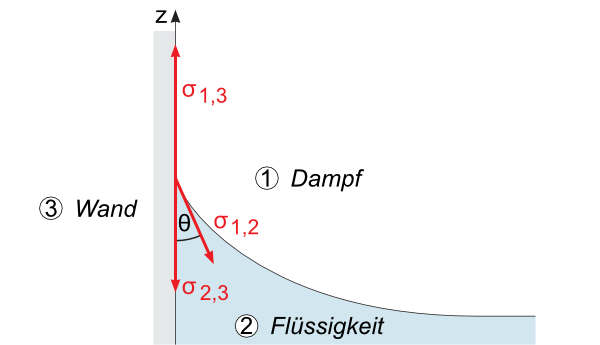
\includegraphics[scale=0.8]{grenzflaechen.png}
\caption{Zur Definition von Grenzflächen\protect\footnotemark}
\end{figure}
\footnotetext{http://lp.uni-goettingen.de/get/text/5065}

Wie man der Grafik entnemen kann können $\sigma_{2,3}$ und $\sigma_{1,3}$ nur in entgegengesetzte Richtung wirken. Also muss
\begin{align*}
 \sigma_{2,3}-\sigma_{1,3}=-\sigma_{1,2}\cdot\cos\theta
\end{align*}
gelten.\newline

Um die Dichten der untersuchten Flüssigkeiten zu bestimmen wird die Mohr'sche Waage verwendet.

\begin{figure} [h]
\centering
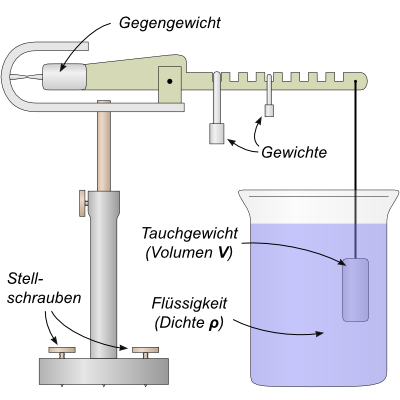
\includegraphics[scale=0.6]{mwaage.png}
\caption{Die Mohrsche Waage\protect\footnotemark}
\end{figure}
\footnotetext{https://lp.uni-goettingen.de/get/text/3638}

Es wird ein Körper mit bekanntem Volumen in die zu untersuchende Flüssigkeit getaucht. Durch die vom Körper verdrängte Flüssigkeit entsteht ein statischer Auftrieb, aus dem nach dem archimedischen Prinzip die Dichte der Flüssigkeit ermittelt werden. Um den entstehenden Auftrieb zu messen wird der Lastarm mittels Gewichten ausgeglichen.
Für eine Flüssigkeit der Dichte $\rho$ gilt bei Gleichgewicht
\begin{align}
 D_{Auftrieb} &= D_{Gewichte} \nonumber\\
\equals  V\cdot\rho\cdot g \cdot r &= \sum_{i=1}^{n}m_i\cdot g\cdot r_i
\end{align}
Somit gilt für zwei Flüssigkeiten
\begin{align}
\frac{V\cdot\rho_2\cdot g \cdot r}{V\cdot\rho_1\cdot g \cdot r} &= \frac{\sum_{i=1}^{n_2}m_{2,i}\cdot g\cdot r_{2,i}}{\sum_{i=1}^{n_1}m_{1,i}\cdot g\cdot r_{1,i}} \nonumber\\
\equals \rho_2 &= \rho_1 \cdot \frac{\sum_{i=1}^{n_2}m_{2,i}\cdot r_{2,i}}{\sum_{i=1}^{n_1}m_{1,i}\cdot r_{1,i}} \label{eq:mohrsche_waage}
\end{align}


\subsection{Dynamische Viskosität}
Die Viskosität $\eta=v\cdot\rho$ eines Fluids ist ein Maß für dessen Zähflüssigkeit.\linebreak

Es existieren zwei verschiedene Strömungsarten die bei Fluiden auftreten können. Die laminare Strömung, bei der keine Turbolenzen auftreten, die Fluide also in Schichten strömen und die turbulente Strömung, bei der Verwirblungen auftreten, so dass die einzelnen Schichten eines Fluids untereinander vermischt werden.\newline
Das Verhältnis von Trägheits- zu Zähigkeitskräften wird durch die dimensionslose  Reynoldzahl Re angegeben. Sie ist ein Maß dafür ob eine Strömung laminar oder turbulent ist. Es gilt
\begin{align*}
  \rm{Re}=\frac{\rho\cdot v\cdot d}{\eta},
\end{align*}
 wobei $\rho$ die Dichte des Fluids, $d$ die Länge des Gegenstandes in dem sich die Strömung befindet und $v$ die durchschnittliche Geschwindigkeit  angibt.\linebreak
 
Verursacht wird die Viskosität von der inneren Reibung $F_r=-\eta\cdot A\cdot\frac{\rm dv}{\rm dr}=-\eta\cdot 2\pi l r\cdot\frac{\rm dv}{\rm dr}$ die entsteht, wenn eine Flüssigkeit durch ein Rohr fließt. Aufgrund des Druckunterschieds $\delta p=(p_1-p_2)$ wirkt ihr dir Kraft $F_p=(p_1-p_2)\cdot\pi\cdot r^2$ entgegen. Mit der Randbedingung v(R)=0 erhält man
\begin{align*}
\Rightarrow\hspace{1cm}-\eta\cdot2 l\cdot\frac{\rm dv}{\rm dr}&=(p_1-p_2)\cdot r \\
\Leftrightarrow\hspace{1.0cm}-\int_r^R\frac{\rm dv}{\rm dr}\rm dr&=\int_r^R\frac{(p_1-p_2)}{2l\cdot\eta} \\
\Leftrightarrow\hspace{2.35cm}v(r)&=\frac{(p_1-p_2)}{4\eta\cdot l}(R^2-r^2)
\end{align*}
Damit lässt sich die gesamte Flüssigkeitsmenge, die pro Zeiteinheit t durch einen Hohlzylinder fließt angeben durch $\rm dV=2\pi\cdot r\cdot v(r)\cdot t\cdot dt$. Integrieren liefert
\begin{align*}
\Rightarrow \hspace*{1cm}\int_0^R\rm dV\,\rm dr&=2\pi\cdot\frac{(p_1-p_2)}{4l\cdot\eta}\cdot t\cdot\int_0^Rr(R^2-r^2)\,\rm dr \\
\Leftrightarrow \hspace*{2.4cm}V&=\frac{\pi\cdot(p_1-p_2)}{8l\cdot\eta}\cdot t\rm,
\end{align*}
woraus man die Hagen-Poiseille Gleichung der laminaren Rohströmung erhält
\begin{align*}
\dot V&=\frac{\pi\cdot(p_1-p_2)}{8l\cdot\eta}\cdot.
\end{align*}
Diese Gleichung sagt aus, wie der Volumenstrom vom Druckgradienten $(p_1-p_2)/l$ und von der Viskosität des Fluids abhängt. Dies zu wissen ist zum Beispiel bei der Wahl des Motoröls im Auto entscheidend. Da man den Rohradius in dem das Öl zufließt nicht verändern kann war es früher notwendig verschiedene Motoröle mit verschiedenen Viskositäten $\eta$ zu verwenden um auf temperaturbedingte Druckunterschiede zu reagieren.

\section{Durchführung}
\label{sec:durchfuehrung}

Um Messfehler durch Verunreinigungen vorzubeugen sind die Kapillare vor jeder Messung gründlich mit 
Lösungsmittel und Wasser zu säubern und anschließend mit der Wasserstrahlpumpe zu trocknen. \\
Der Radius R jeder Kapillare ist mindestens dreimal mit Hilfe des Mikroskops zu bestimmen.\\

\subsection{Teilversuch 1: Kapillarität}
Die zu untersuchenden Flüssigkeiten, destilliertes Wasser, Methanol und Ethylenglykol werden in ausreichender Menge in Bechergläser gegeben. Jede der Kapillaren wird in die Flüssigkeiten getaucht und dann soweit wieder herausgehoben, dass sich der Nullpunkt der Messskala auf gleichem Niveau mit dem Flüssigkeitsspiegel der Flüssigkeit im Becherglas befindet. Mit Hilfe der Skala ist dann der Höhenunterschied $h_kap$ der Flüssigkeitsspiegel zu bestimmen. Dies wird für jedes Kapillar und jede Flüssigkeit mindestens dreimal wiederholt. \\
Die Dichte $rho$ der Flüssigkeiten ist mit Hilfe der Mohrschen Waage zu bestimmen, wobei darauf geachtet werden sollte, dass der Probekörper trocken und sauber ist, bevor er in die Flüssigkeit getaucht wird und dass er in diese für die Messung dann vollständig eingetaucht ist.\\

\subsection{Teilversuch 2: Viskosität}
\begin{figure}
\centering
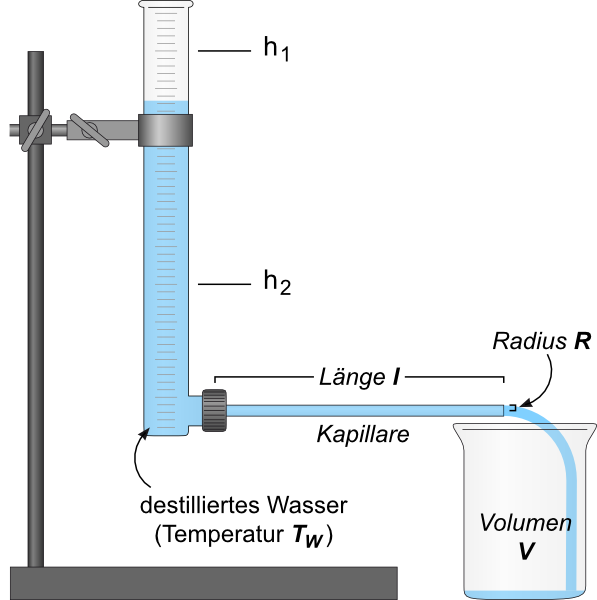
\includegraphics[scale=0.7]{Hagen-Poiseuille.png}
\caption{Versuchsaufbau: $\left($ Hagen-Poiseuillesches Gesetz $\right)$}
\end{figure}
Zu messen sind die Temperatur $T_W$ des destillierten Wassers, die Länge der Kapillaren $l$, sowie das Volumen des Glasgefäßes zwischen den Strichmarken 50 und 45.\\
\begin{itemize}
\item Für jedes der drei Kapillare ist die Ausflusszeit $t_A$ von destilliertem Wasser zwischen den Strichmarken  50 und 45 zu bestimmen.
\item Für die Kapillare mit dem geringsten Durchmesser sind mindestens 10 Werte der Abflusszeit $t \left( h \right)$ $\left( \textrm{in Abhängigkeit der Höhe} h \textrm{der Wassersäule} \right)$ zu bestimmen.
\end{itemize}

\section{Auswertung}
\label{sec:auswertung}

In der Tabelle \ref{tab:l_kap} und Tabelle \ref{tab:d_kap} sind die gemessenen Längen $l$ und Durchmesser $d$ der Kapillare.
Aus den Werten in Tabelle \ref{tab:mohrsche_waage} und der Formel \eqref{eq:mohrsche_waage} folgen die relativen Dichten von destilliertem Wasser, Methanol und Ethylenglykol und mit der Vorraussetzung $\rho _{Wasser} = 10^{3}\cdot\kilogramm\cdot\meter^{-3}$ die Dichten in Tabelle \ref{tab:dichte}.

\begin{wraptable}{r}{5cm}[!h]
\centering
\begin{tabular}{r|l}
    Kapillar & $l[\milli\meter]$\\
    \hline
    Rot & $231(1)$\\
    Blau & $220(1)$\\
    Grün & $228(1)$\\
    
 \end{tabular} 
 \caption{\label{tab:l_kap}Länge $l$ der Kapillare}
\end{wraptable}

\begin{table}[!h]
\centering
\begin{tabular}{r|c|c|c||c|c}
    Kapillar & Messung 1 & Messung 2 & Messung 3 & Verwendet & rel. Fehler\\
    \hline
    Rot & $69(2)$ & $84(2)$ & $86(2)$ & $85(2)$ & $ 2.4\%$\\
    Blau & $116(2)$ & $117(2)$ & $117(2)$ & $117(2)$ & $ 1.7\%$\\
    Grün & $181(2)$ & $179(2)$ & $181(2)$ & $180(2)$ & $ 1.1\%$\\
    
 \end{tabular} 
 \caption{\label{tab:d_kap} Durchmesser der Kapillare in $ 10^{-5} \meter$}
\end{table}

\begin{table}[!h]
\centering
\begin{tabular}{r|c|c|c|c|c|c|c|c|c}
    Auslenkung $r[\centi\meter]$ & 1 & 2 & 3 & 4 & 5 & 6 & 7 & 8 & 9\\
    \hline
    \hline
    Wasser & & & & & & & & $11$ & $100$ \\
    \hline
    Methanol & & & $1$ & $10$ & & & & $100$ & \\
    \hline
    Ethylenglykol & & & & $100$ & & $100$ & & $10$ & \\
    
 \end{tabular} 
 \caption{\label{tab:mohrsche_waage}Gewichteverteilung bei der Mohrschen Waage}
\end{table}

\begin{table}[!h]
\centering
\begin{tabular}{r|c}
    Flüssigkeit & Dichte $\rho [\kilogramm\cdot\meter^{-3}]$\\
    \hline
    Wasser & $1.00\cdot 10^{3}$\\
    \hline
    Methanol & $ 0.85\cdot 10^{3}$\\
    \hline
    Ethylenglykol & $ 1.09 \cdot 10^{3}$\\
    
 \end{tabular} 
 \caption{\label{tab:dichte}Dichte}
\end{table}

\subsection{Kapillarität}

Die Messwerte der Höhenunterschiede $h_{Kap}$ zur Bestimmung der Kapillarität sind in Tabelle \ref{tab:h_kap_was} für destilliertes Wasser, in Tabelle \ref{tab:h_kap_met} für Methanol und in Tabelle \ref{tab:h_kap_eth} für Ethylenglykol aufgeführt.
Aus diesen Messwerten ergeben sich nach den Formeln \eqref{eq:oberflaechenspannung} die Werte für die Oberflächenspannung $\sigma$  in der Tabelle \ref{tab:oberflaechenspannung}, sowie in der Grafik \ref{img:oberflaechenspannung}.
Für die Berechnung der Fehler in der Oberflaechenspannung gilt
\begin{align}
  \frac{\sigma_\sigma}{\sigma} = \sqrt{\left(\frac{\sigma_{R}}{R}\right)^2 + \left(\frac{\sigma_{\rho}}{\rho}\right) ^2 + \left(\frac{\sigma_{h}}{h}\right)^2} 
\end{align}

\begin{table}
\centering
\begin{tabular}{r|c|c|c}
    Kapillar & Messung 1 & Messung 2 & Messung 3\\
    \hline
    Rot & $35$ & $37$ & $38$ \\
    Blau & $9$ & $23$ & $24$ \\
    Grün & $15$ & $17$ & $15$ \\
    
 \end{tabular} 
 \caption{\label{tab:h_kap_was}$h_{Kap} \rm{in} \milli\meter$ für destilliertes Wasser mit einem Fehler von $\pm 1\milli\meter$}
\end{table}

\begin{table}
\centering
\begin{tabular}{r|c|c|c}
    Kapillar & Messung 1 & Messung 2 & Messung 3\\
    \hline
    Rot & $15$ & $14$ & $14$\\
    Blau & $10$ & $10$ & $11$ \\
    Grün & $6$ & $6$ & $7$\\
    
 \end{tabular} 
 \caption{\label{tab:h_kap_met}$h_{Kap} \rm{in} \milli\meter$ für Methanol mit einem Fehler von $\pm 1\milli\meter$}
\end{table}

\begin{table}
\centering
\begin{tabular}{r|c|c|c}
    Kapillar & Messung 1 & Messung 2 & Messung 3\\
    \hline
    Rot & $22$ & $22$ & $24$\\
    Blau & $20$ & $16$ & $15$ \\
    Grün & $10$ & $10$ & $11$\\
    
 \end{tabular} 
 \caption{\label{tab:h_kap_eth}$h_{Kap} \rm{in} \milli\meter$ für Ethylenglykol mit einem Fehler von $\pm 1\milli\meter$}
\end{table}

\begin{table}
\centering
\begin{tabular}{r|c|c|c}
    Kapillar/Messung & $\sigma _{Wasser}$ & $\sigma _{Methanol}$ & $\sigma _{Ethylenglykol}$\\
    \hline
    Rot 1 & $ 73(3)$ & $ 26.5$ & $ 50.0$\\
    Rot 2 & $ 77(3)$ & $ 24.8$ & $ 50.0$\\
    Rot 3 & $ 79(3)$ & $ 24.8$ & $ 54.5$ \\
    \hline
    Blau 1 & $ 26(3)$ & $ 24.4$ & $ 62.5$ \\
    Blau 2 & $ 66(3)$ & $ 24.4$ & $ 50.0$ \\
    Blau 3 & $ 69(3)$ & $ 26.8$ & $ 46.9$ \\
    \hline
    Grün 1 & $ 66(5)$ & $ 22.5$ & $ 48.1$ \\
    Grün 2 & $ 75(5)$ & $ 22.5$ & $ 48.1$ \\
    Grün 3 & $ 66(5)$ & $ 26.3$ & $ 52.9$ \\
    
 \end{tabular} 
 \caption{\label{tab:oberflaechenspannung}Oberflächenspannung $\sigma$ in $ $}
\end{table}


\subsection{Viskosität}


\begin{table}
\centering
\begin{tabular}{rl}
    Kapillar & $t_A$\\
    \hline
    Rot & 67\\
    Blau & 20 \\
    Grün & 6\\
    
 \end{tabular} \label{tab:t_A}
 \caption{Ausflusszeit $t_A$ von $20.5\milli\liter$ destilliertem Wasser bei $50\centi\meter$ Füllhöhe}
\end{table}



\begin{table}
\centering
\begin{tabular}{r|c|c|c|c|c|c|c|c|c|c}
    Messung & 1 & 2 & 3 & 4 & 5 & 6 & 7 & 8 & 9 & 10\\
    \hline
    \hline
    $h_1[\centi\meter]$ & $49$ & $45$ & $40$ & $35$ & $30$ & $50$ & $40$ & $50$ & $46$ & $42$  \\
    \hline
    $h_2[\centi\meter]$ & $45$ & $40$ & $35$ & $30$ & $25$ & $40$ & $30$ & $43.5$ & $42.5$ & $38.5$ \\
    \hline
    $t[\second]$ & $52$ & $75$ & $83$ & $99$ & $112$ & $142$ & $182$ & $45$ & $49$ & $54$ \\
    
 \end{tabular} \label{tab:werte}
 \caption{Länge $l$ der Kapillare in $\milli\meter$}
\end{table}


\section{Diskussion}
\label{sec:diskussion}

\end{document}
